\section{Phân tích khám phá dữ liệu}

\subsection{Aggregate sales và stockout}

Hai hình đầu tiên cho thấy bức tranh tổng quát của dữ liệu: aggregate observed sales theo thời gian và stockout rate theo thời gian. Đây là hai đồ thị quan trọng nhất để motivate bài toán. Nếu chỉ nhìn aggregate sales, các giai đoạn giảm bán có thể bị hiểu là demand giảm. Nhưng khi đặt cạnh stockout rate, ta thấy cần phân biệt giữa demand thấp và availability thấp.


\begin{figure}[H]
    \centering
    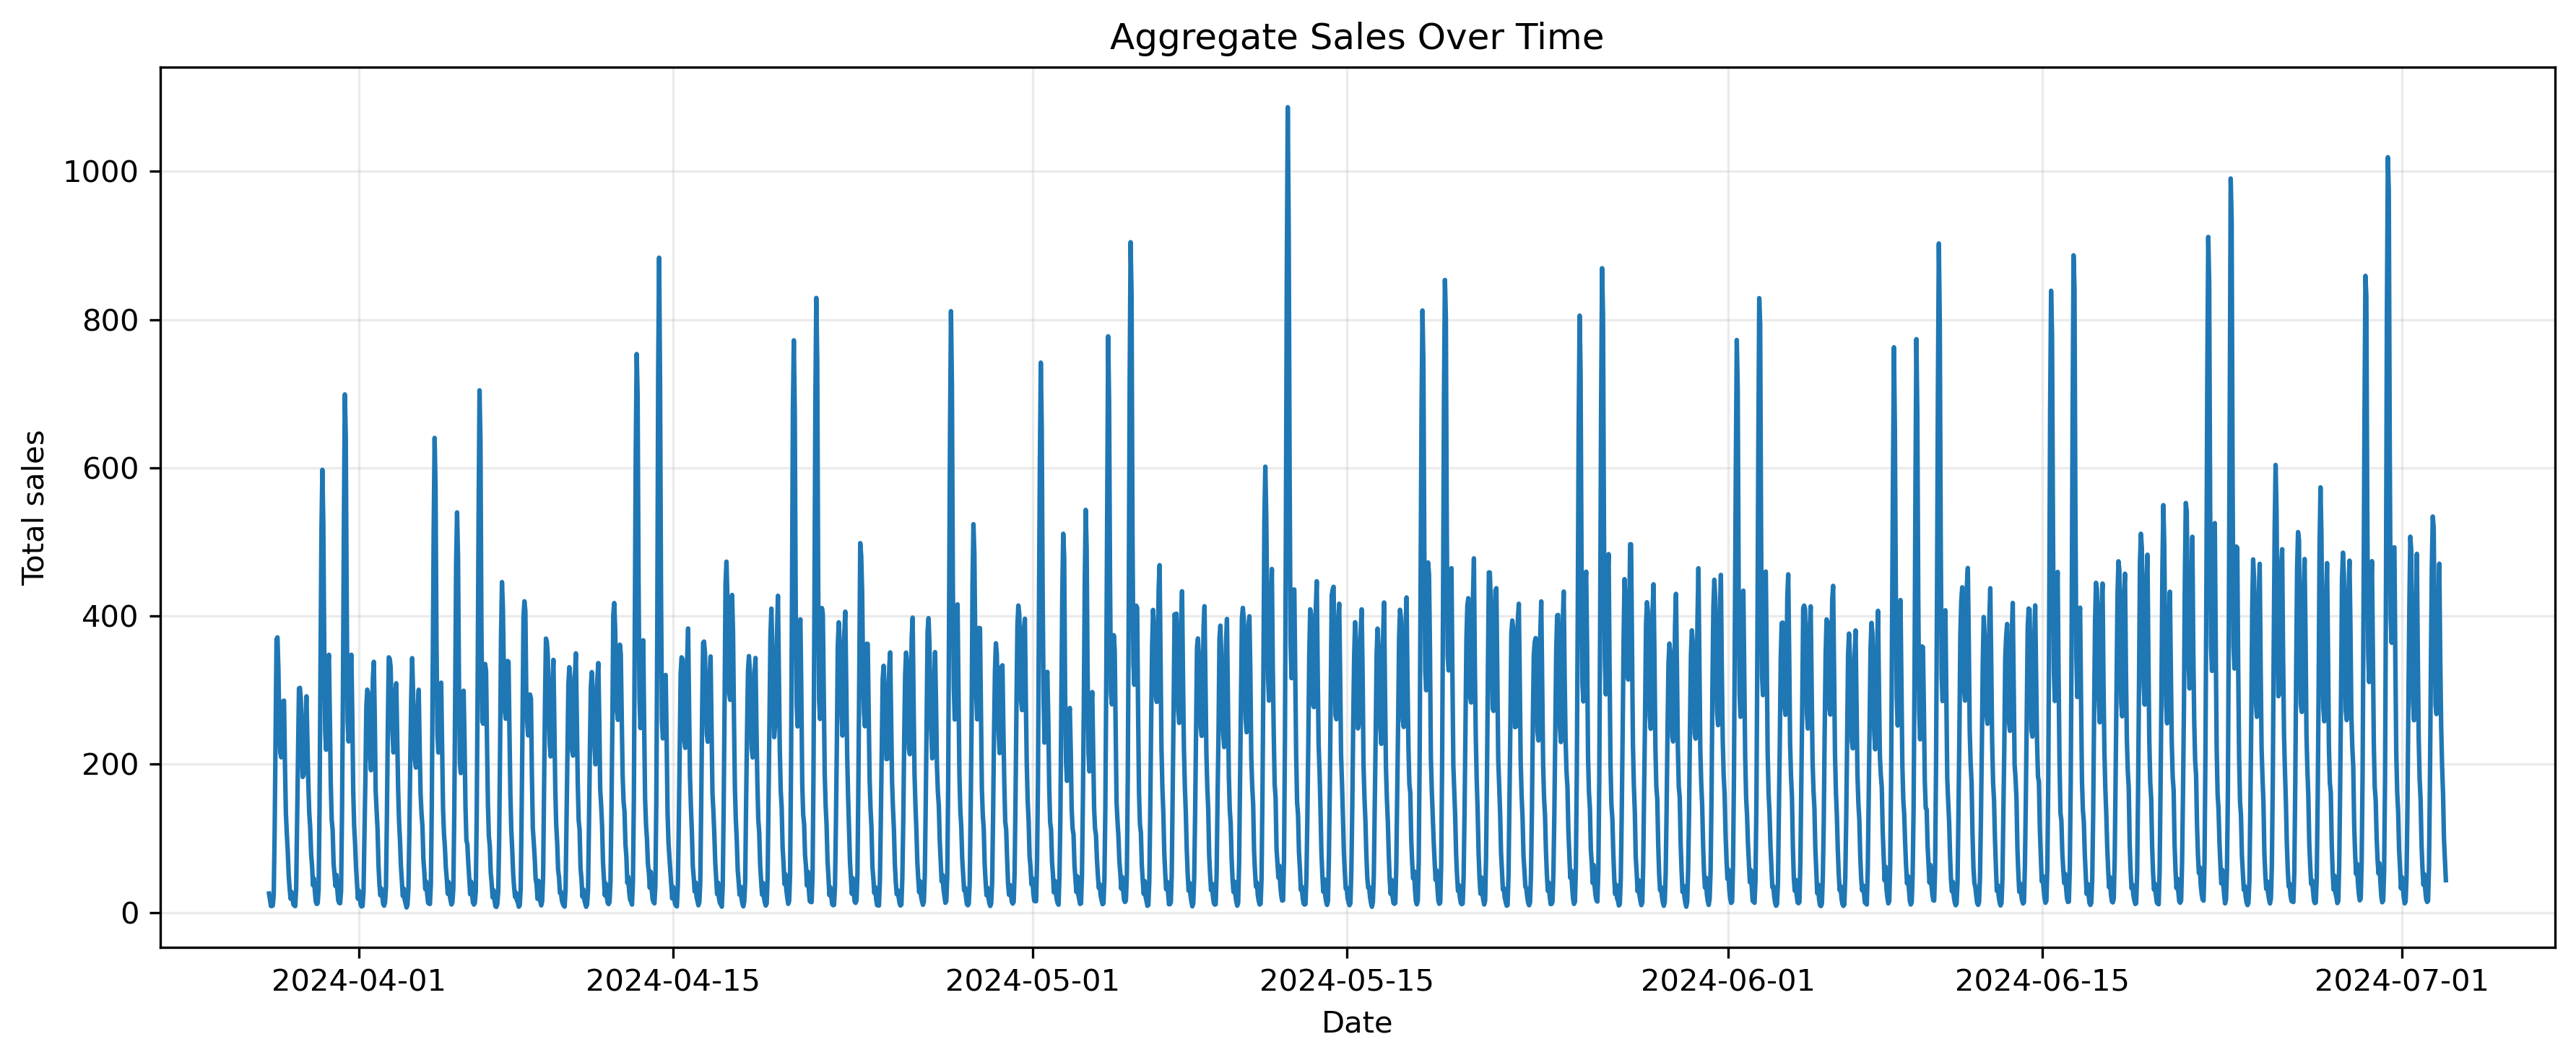
\includegraphics[width=0.92\linewidth]{figures/aggregate_sales_over_time.png}
    \caption{Tổng observed sales theo giờ.}
    \label{fig:long-aggregate-sales}
\end{figure}



\begin{figure}[H]
    \centering
    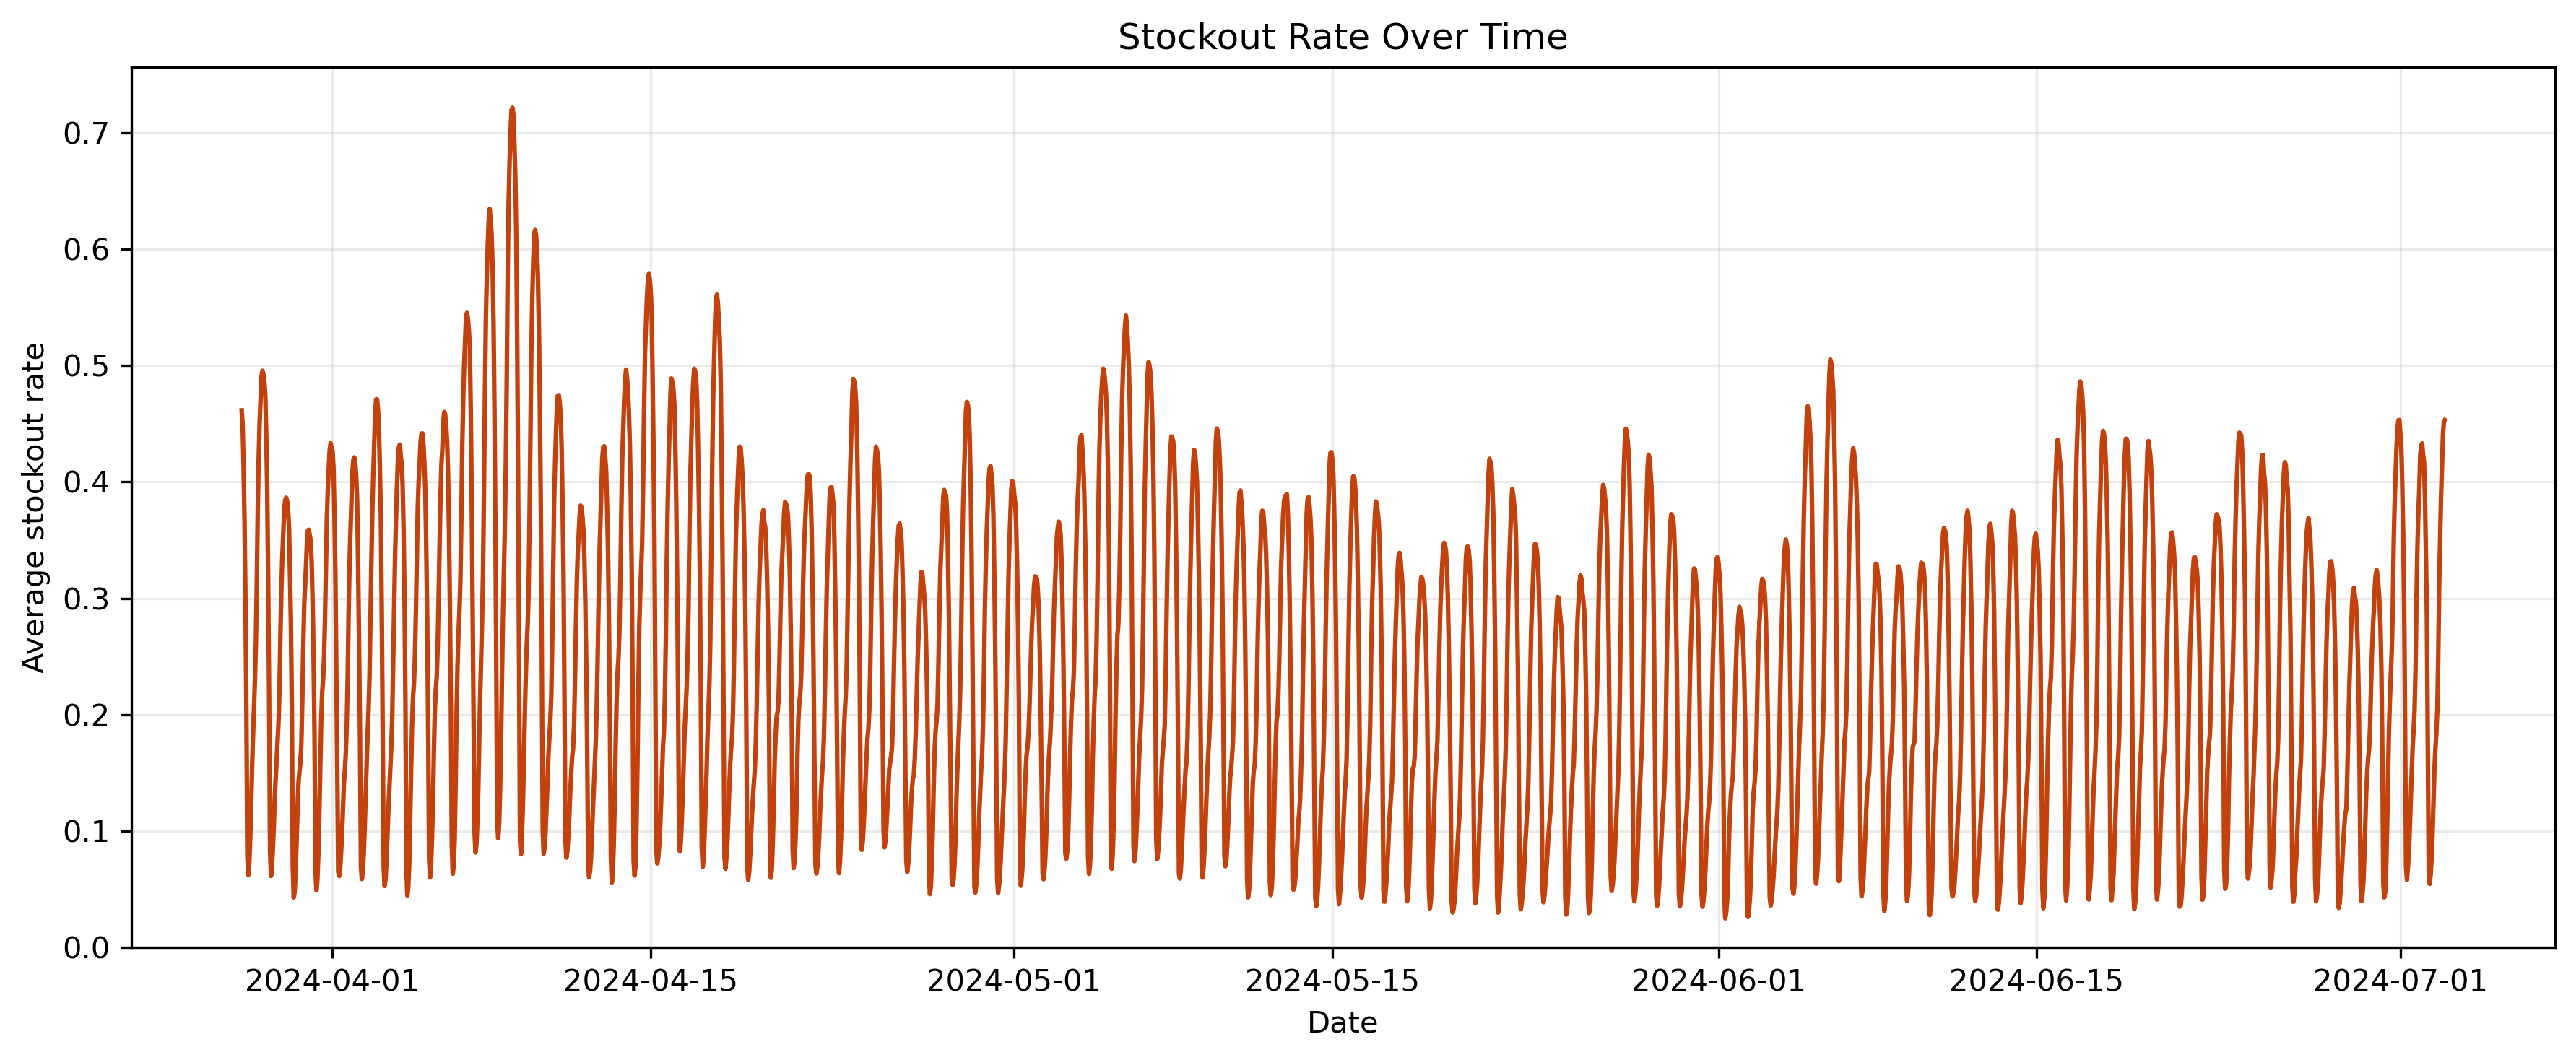
\includegraphics[width=0.92\linewidth]{figures/stockout_rate_over_time.png}
    \caption{Tỷ lệ stockout theo giờ.}
    \label{fig:long-stockout-rate}
\end{figure}


\subsection{Phân phối sales}

Phân phối sale amount cho thấy dữ liệu bán lẻ rất thưa, nhiều giá trị nhỏ và zero, đồng thời có các spike lớn. Đây là lý do không dùng MAPE đơn thuần làm metric chính; WAPE, MAE và RMSE phù hợp hơn vì ổn định hơn khi dữ liệu có nhiều zero.


\begin{figure}[H]
    \centering
    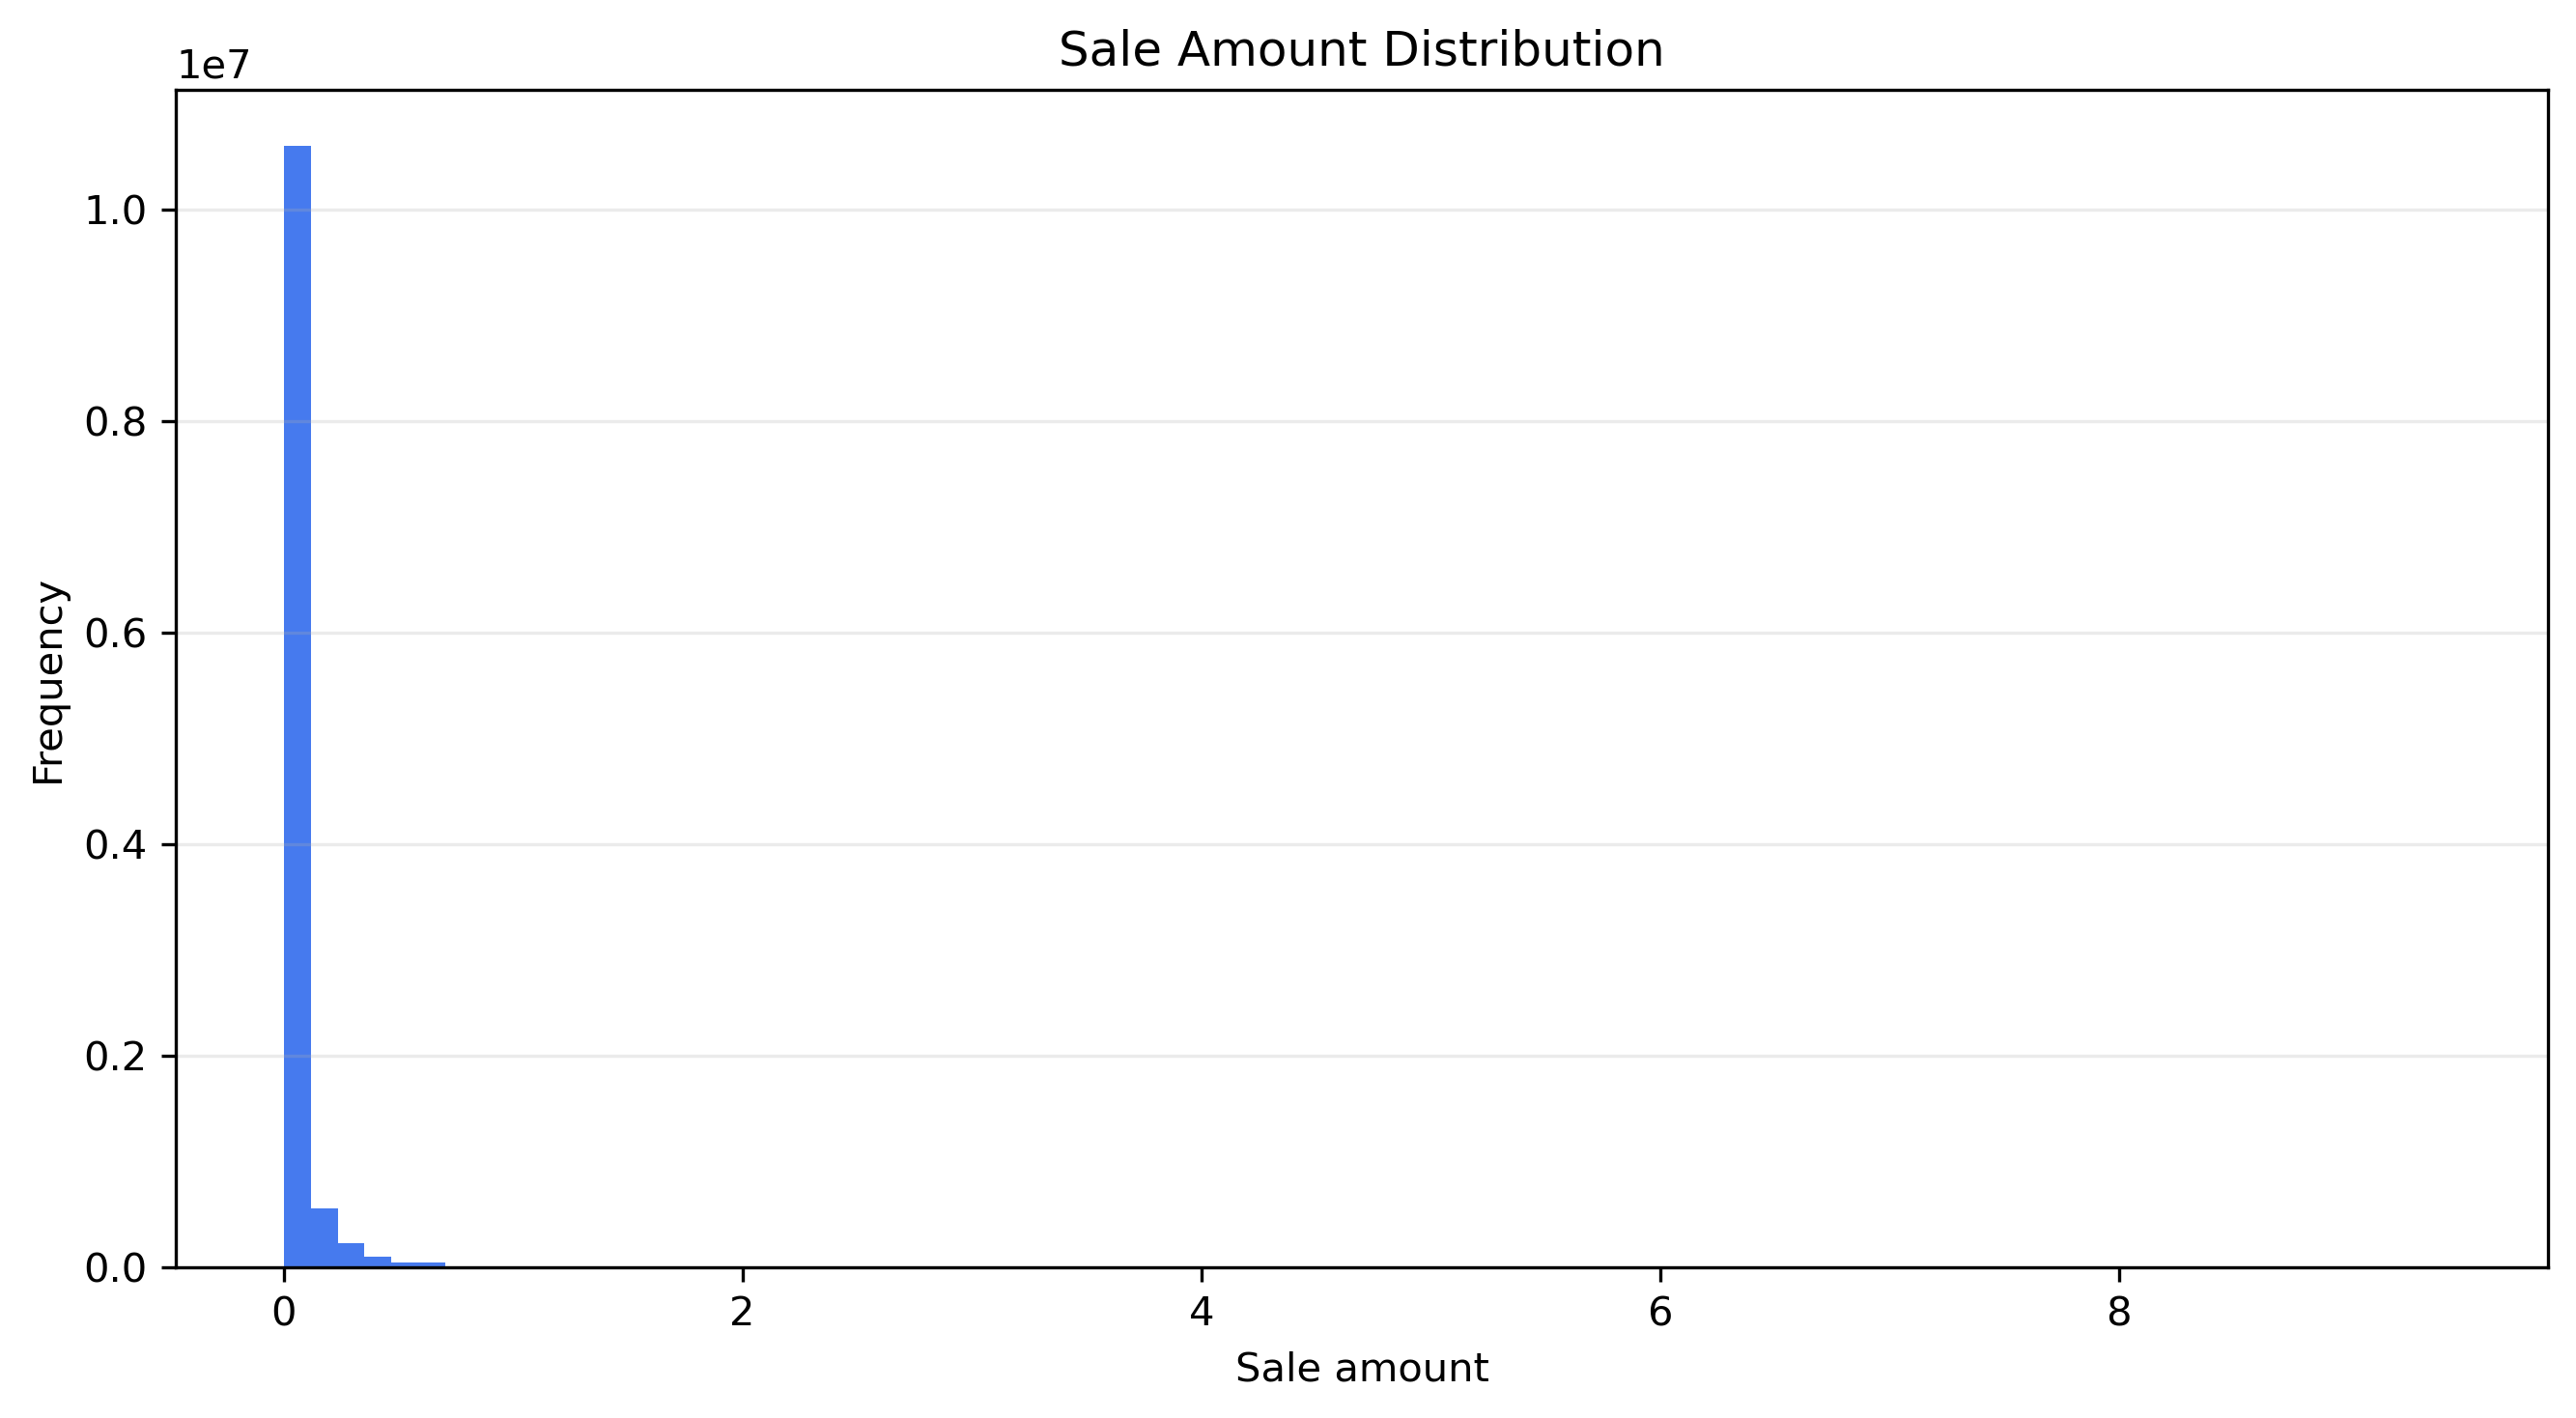
\includegraphics[width=0.78\linewidth]{figures/sale_amount_distribution.png}
    \caption{Phân phối sale amount hourly.}
    \label{fig:long-sale-dist}
\end{figure}



\begin{figure}[H]
    \centering
    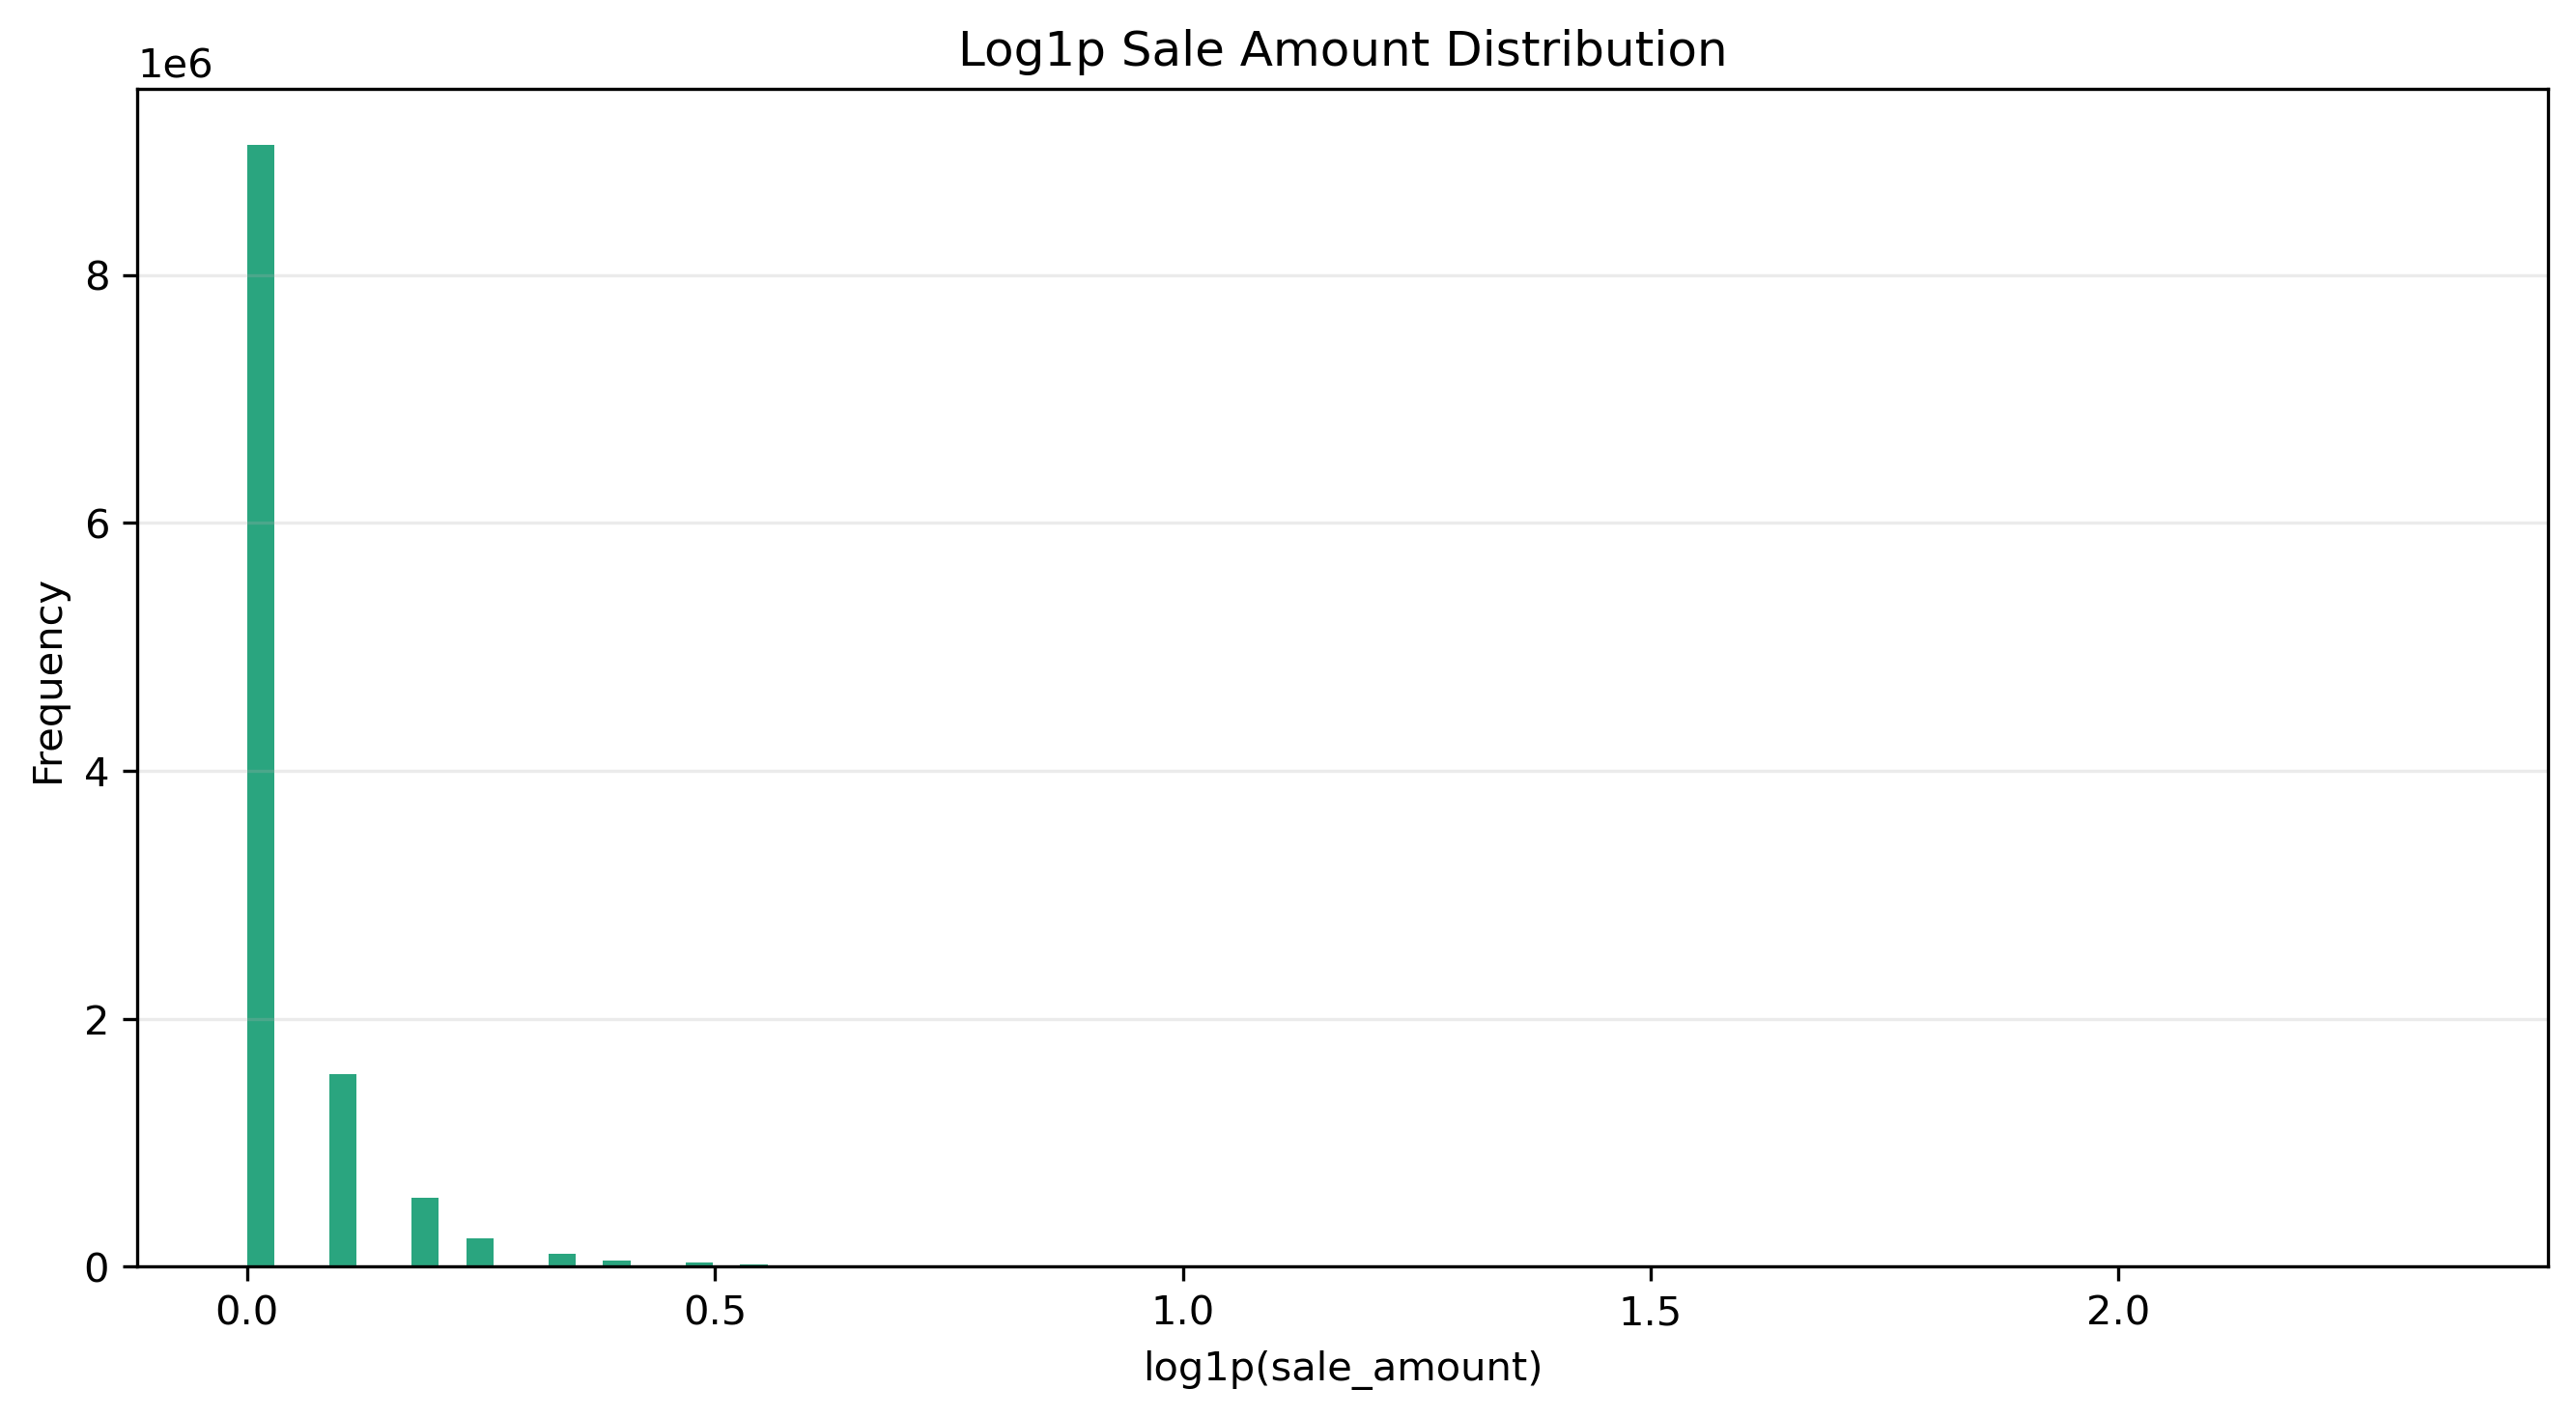
\includegraphics[width=0.78\linewidth]{figures/log_sale_amount_distribution.png}
    \caption{Phân phối log1p sale amount hourly.}
    \label{fig:long-log-sale-dist}
\end{figure}


\subsection{Seasonality theo giờ và theo tuần}

Seasonality là insight quan trọng nhất của dữ liệu. Sales thay đổi theo giờ trong ngày và theo thứ trong tuần. Điều này giải thích vì sao seasonal naive theo tuần là baseline rất mạnh ở phần kết quả. Trong bối cảnh bán lẻ, pattern tuần phản ánh hành vi mua sắm lặp lại của khách hàng, lịch hoạt động của cửa hàng và các chu kỳ khuyến mãi.


\begin{figure}[H]
    \centering
    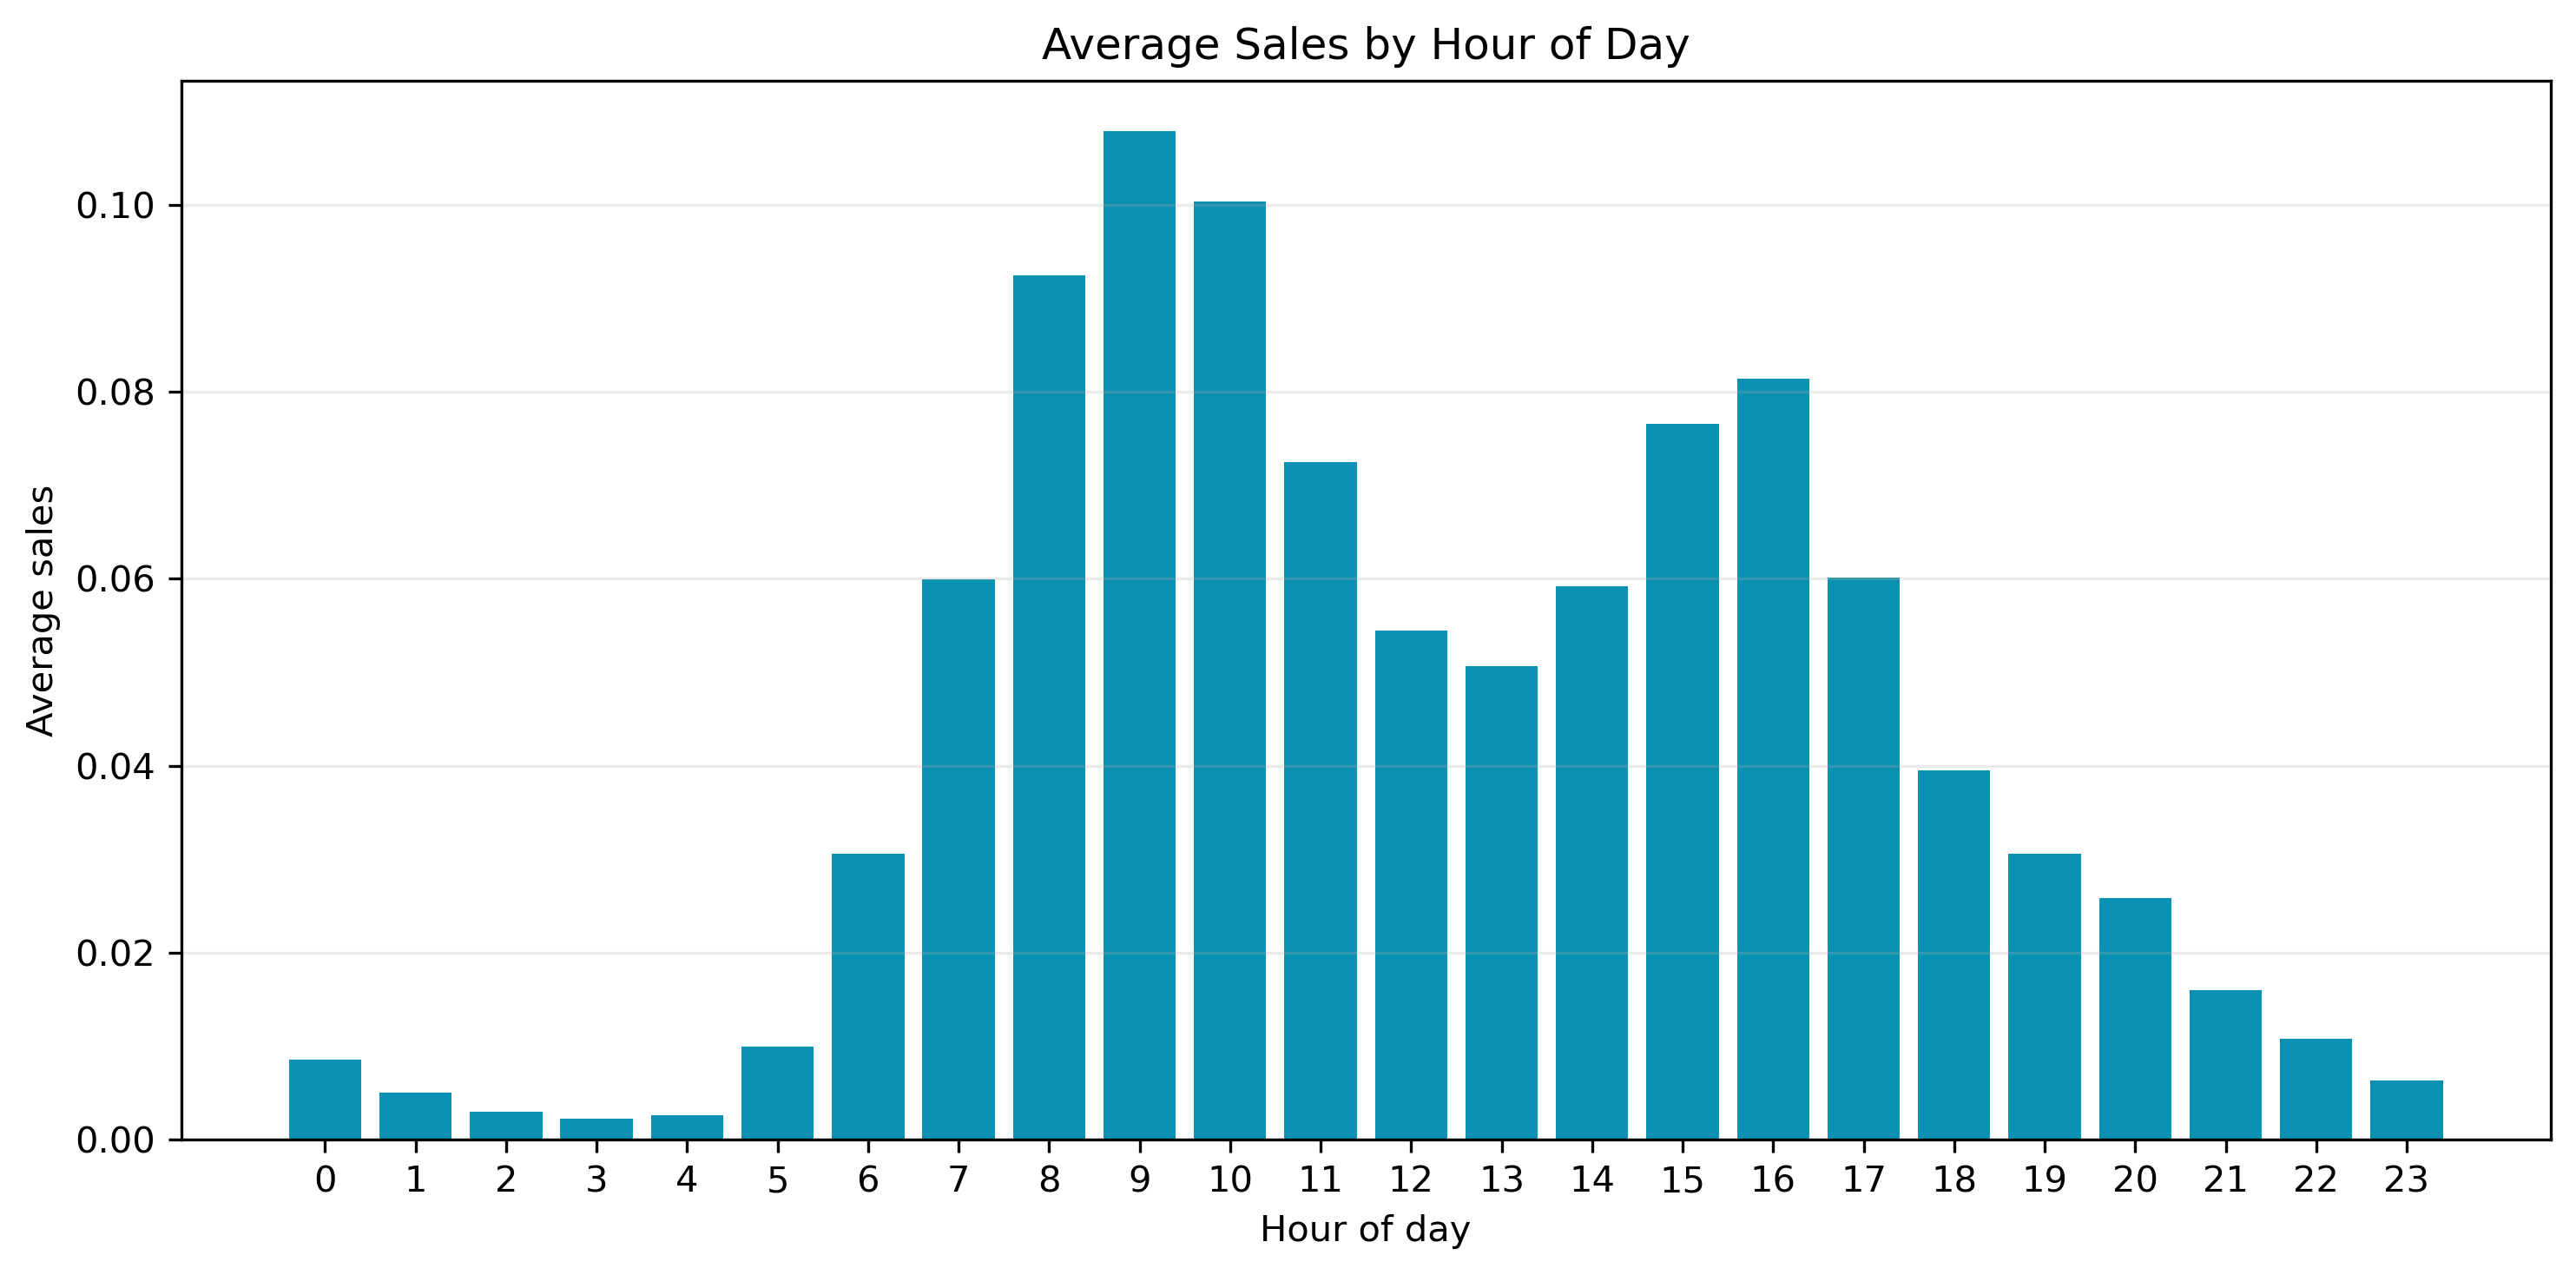
\includegraphics[width=0.78\linewidth]{figures/sales_by_hour_of_day.png}
    \caption{Sales trung bình theo giờ trong ngày.}
    \label{fig:long-hour-seasonality}
\end{figure}



\begin{figure}[H]
    \centering
    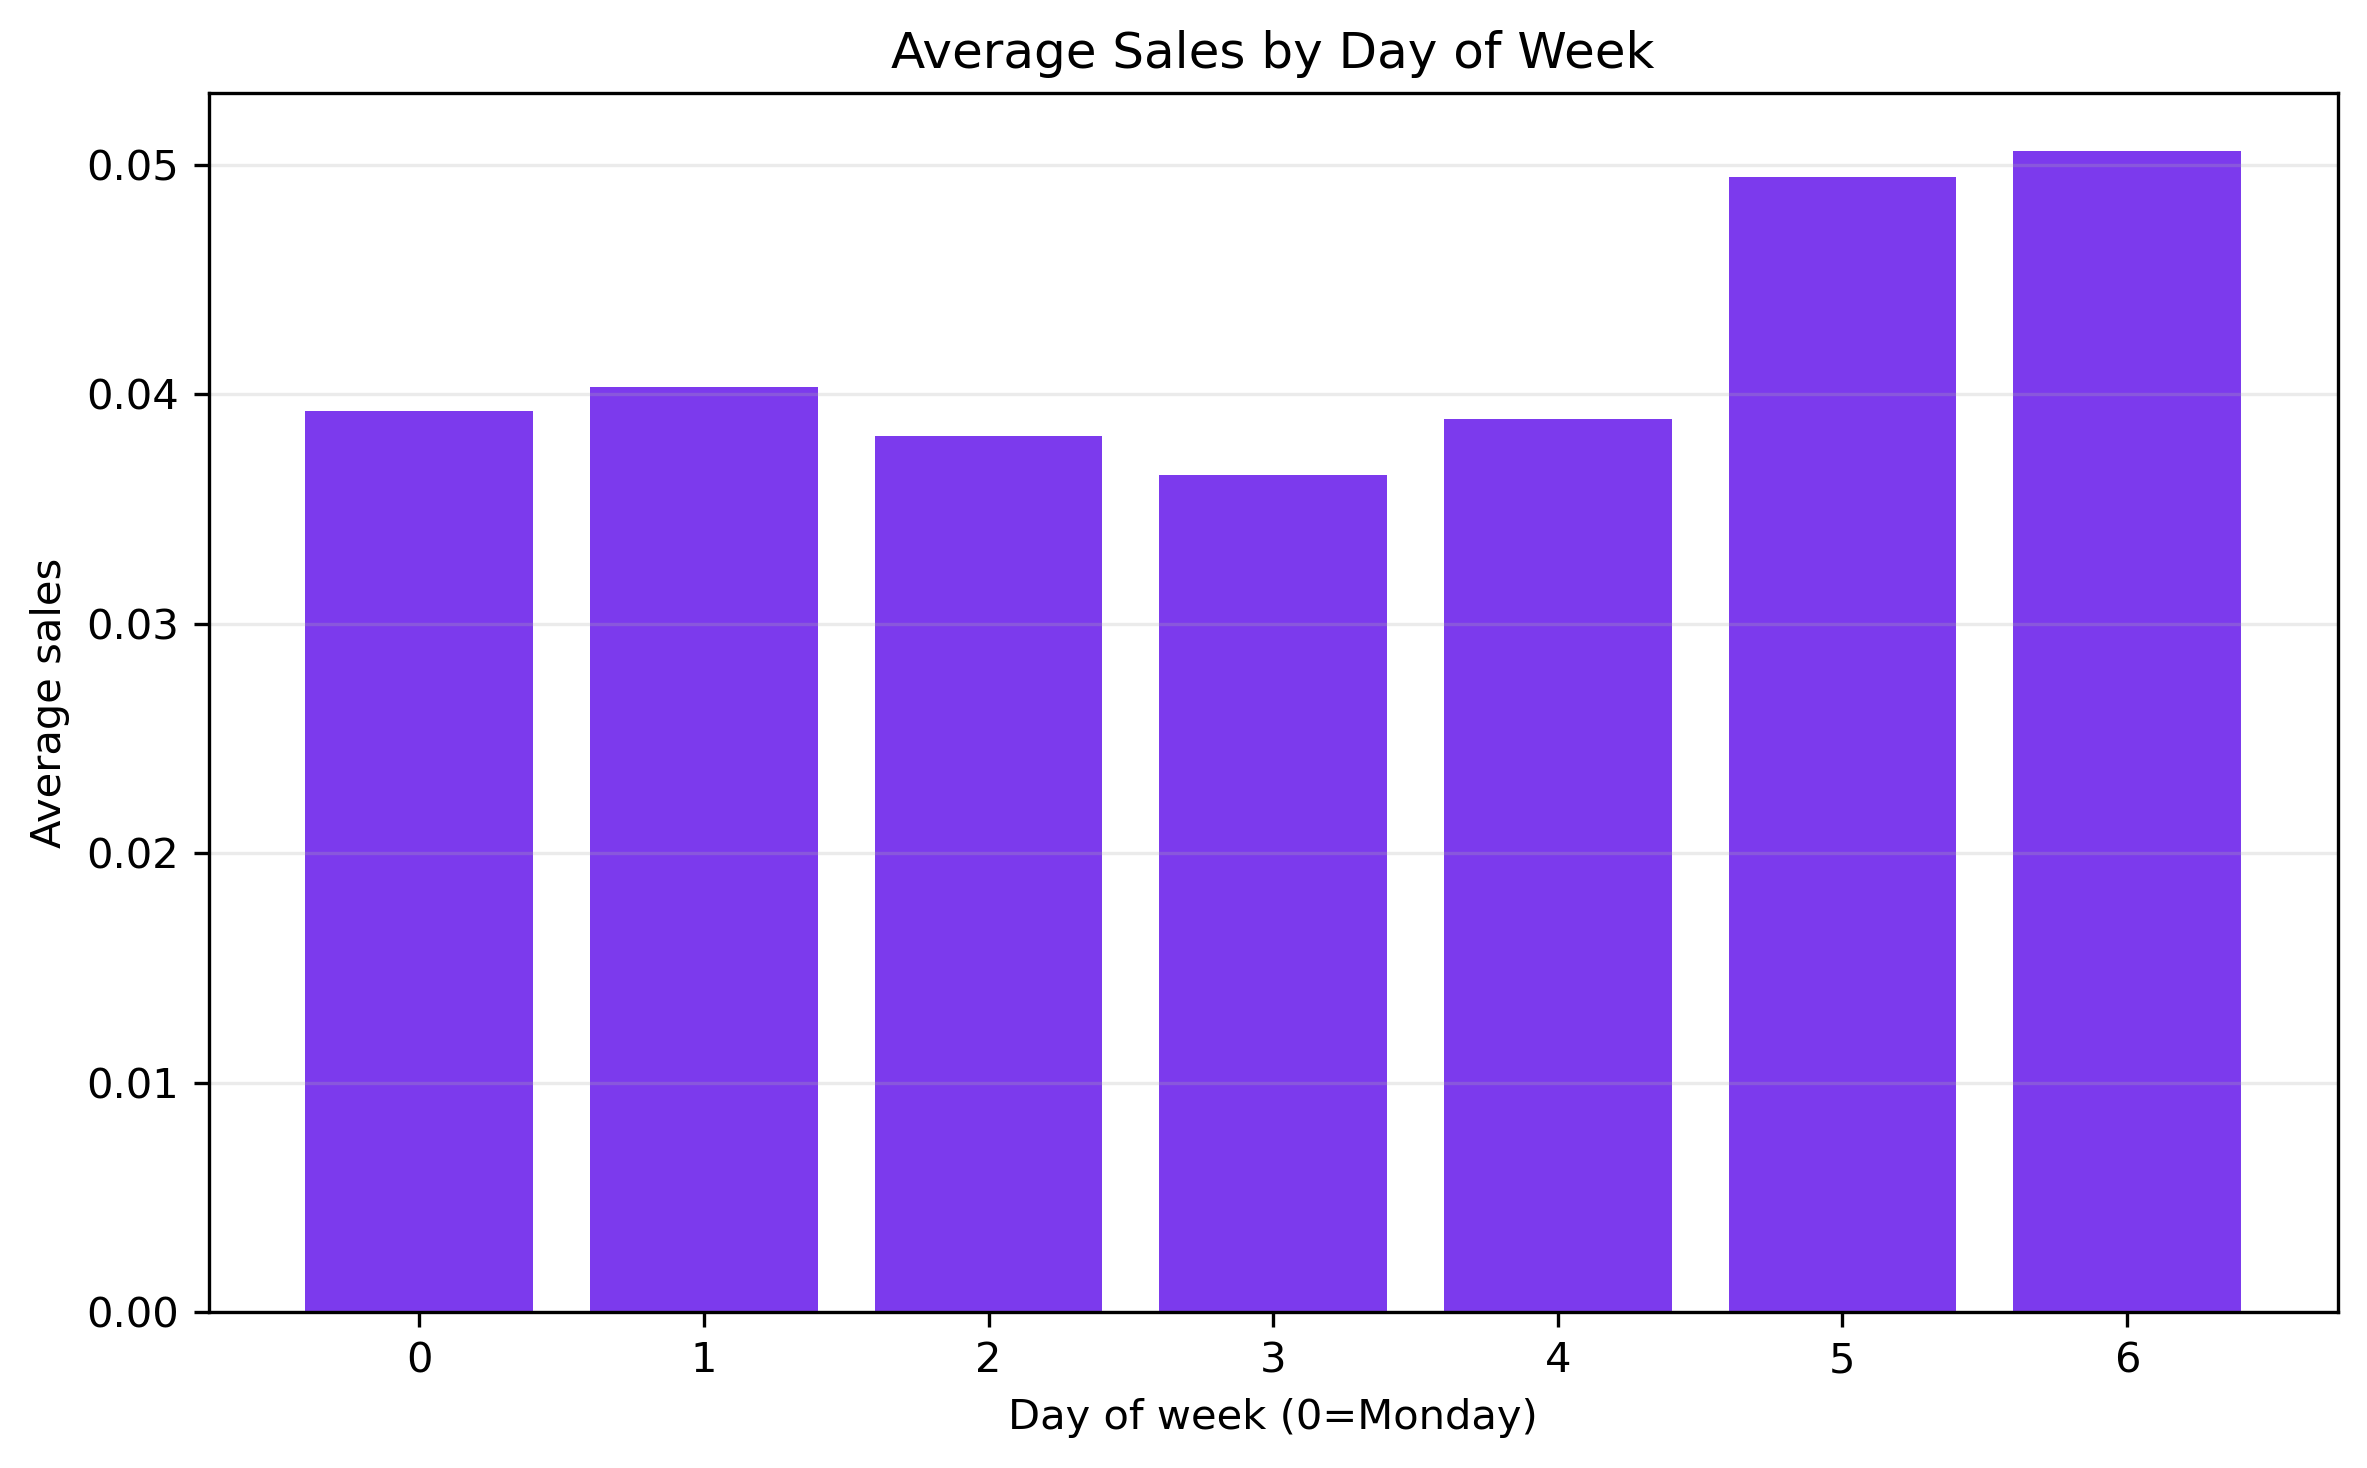
\includegraphics[width=0.78\linewidth]{figures/sales_by_day_of_week.png}
    \caption{Sales trung bình theo thứ trong tuần.}
    \label{fig:long-dow-seasonality}
\end{figure}


\subsection{Chuỗi đại diện}

Để không plot hàng nghìn chuỗi, báo cáo chọn ba chuỗi đại diện: high-volume, intermittent và stockout-heavy. Ba nhóm này minh họa ba kiểu khó khác nhau của forecasting: chuỗi lớn có pattern rõ, chuỗi thưa có nhiều zero, và chuỗi stockout-heavy có observed sales bị censor nặng.


\begin{table}[H]
\centering
\caption{Ba chuỗi đại diện}
\label{tab:long-representative}
\resizebox{0.86\linewidth}{!}{%
\begin{tabular}{lllll}
\toprule
series\_id & type & total\_sales & stockout\_rate & n\_obs \\
\midrule
4\_11\_267 & high\_volume & 1,896 & 0.6070 & 2328 \\
3\_793\_550 & intermittent & 49.7000 & 0.1907 & 2328 \\
5\_6\_757 & stockout\_heavy & 48.4000 & 0.7371 & 2328 \\
\bottomrule
\end{tabular}
}
\end{table}



\begin{figure}[H]
    \centering
    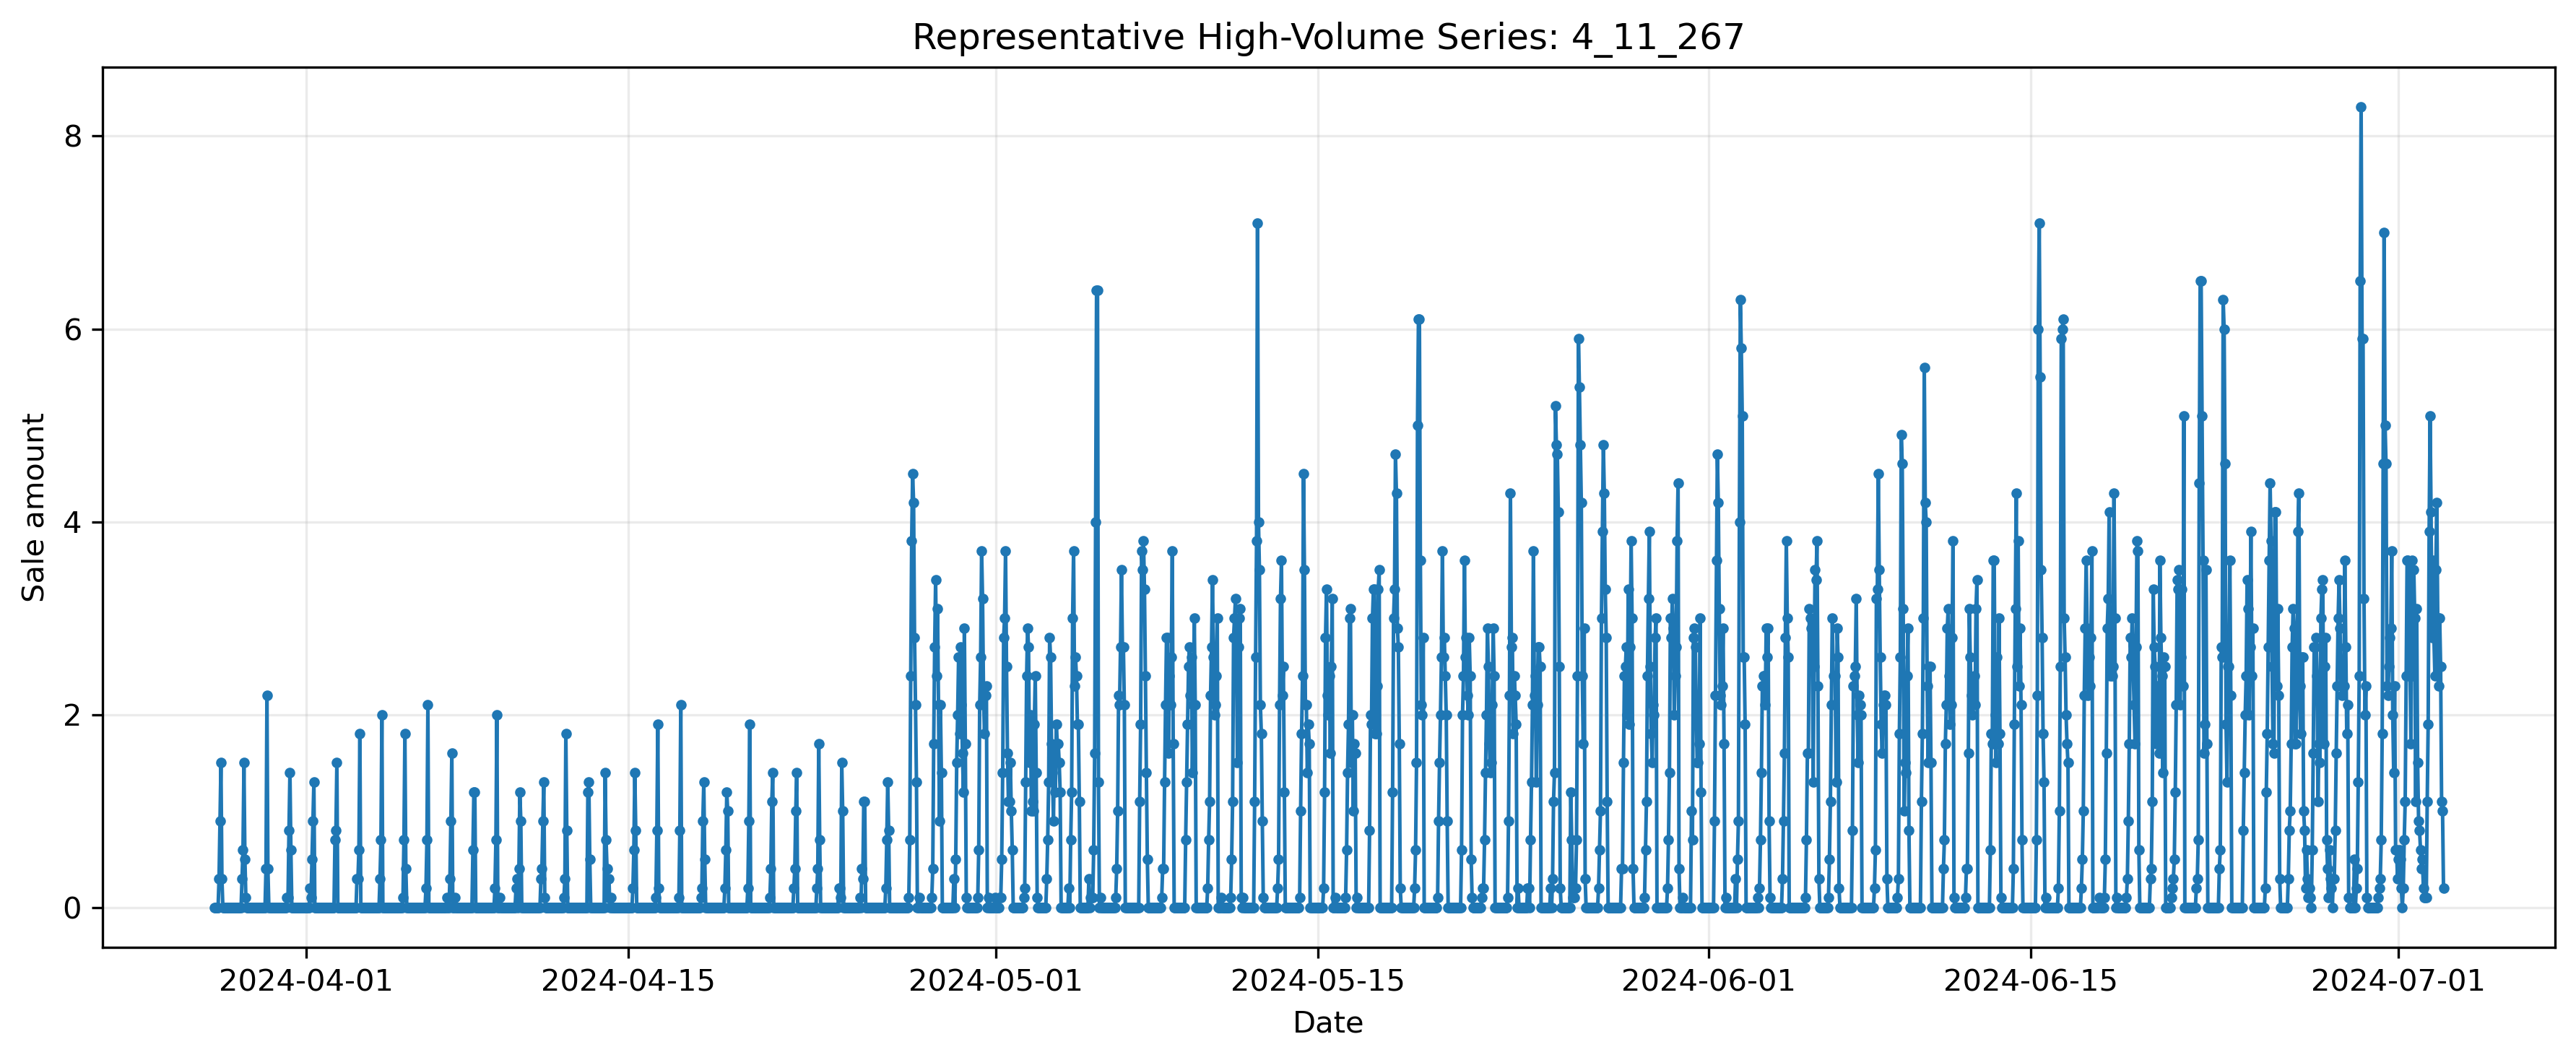
\includegraphics[width=0.92\linewidth]{figures/representative_series_high_volume.png}
    \caption{Chuỗi đại diện high-volume.}
    \label{fig:long-rep-high}
\end{figure}



\begin{figure}[H]
    \centering
    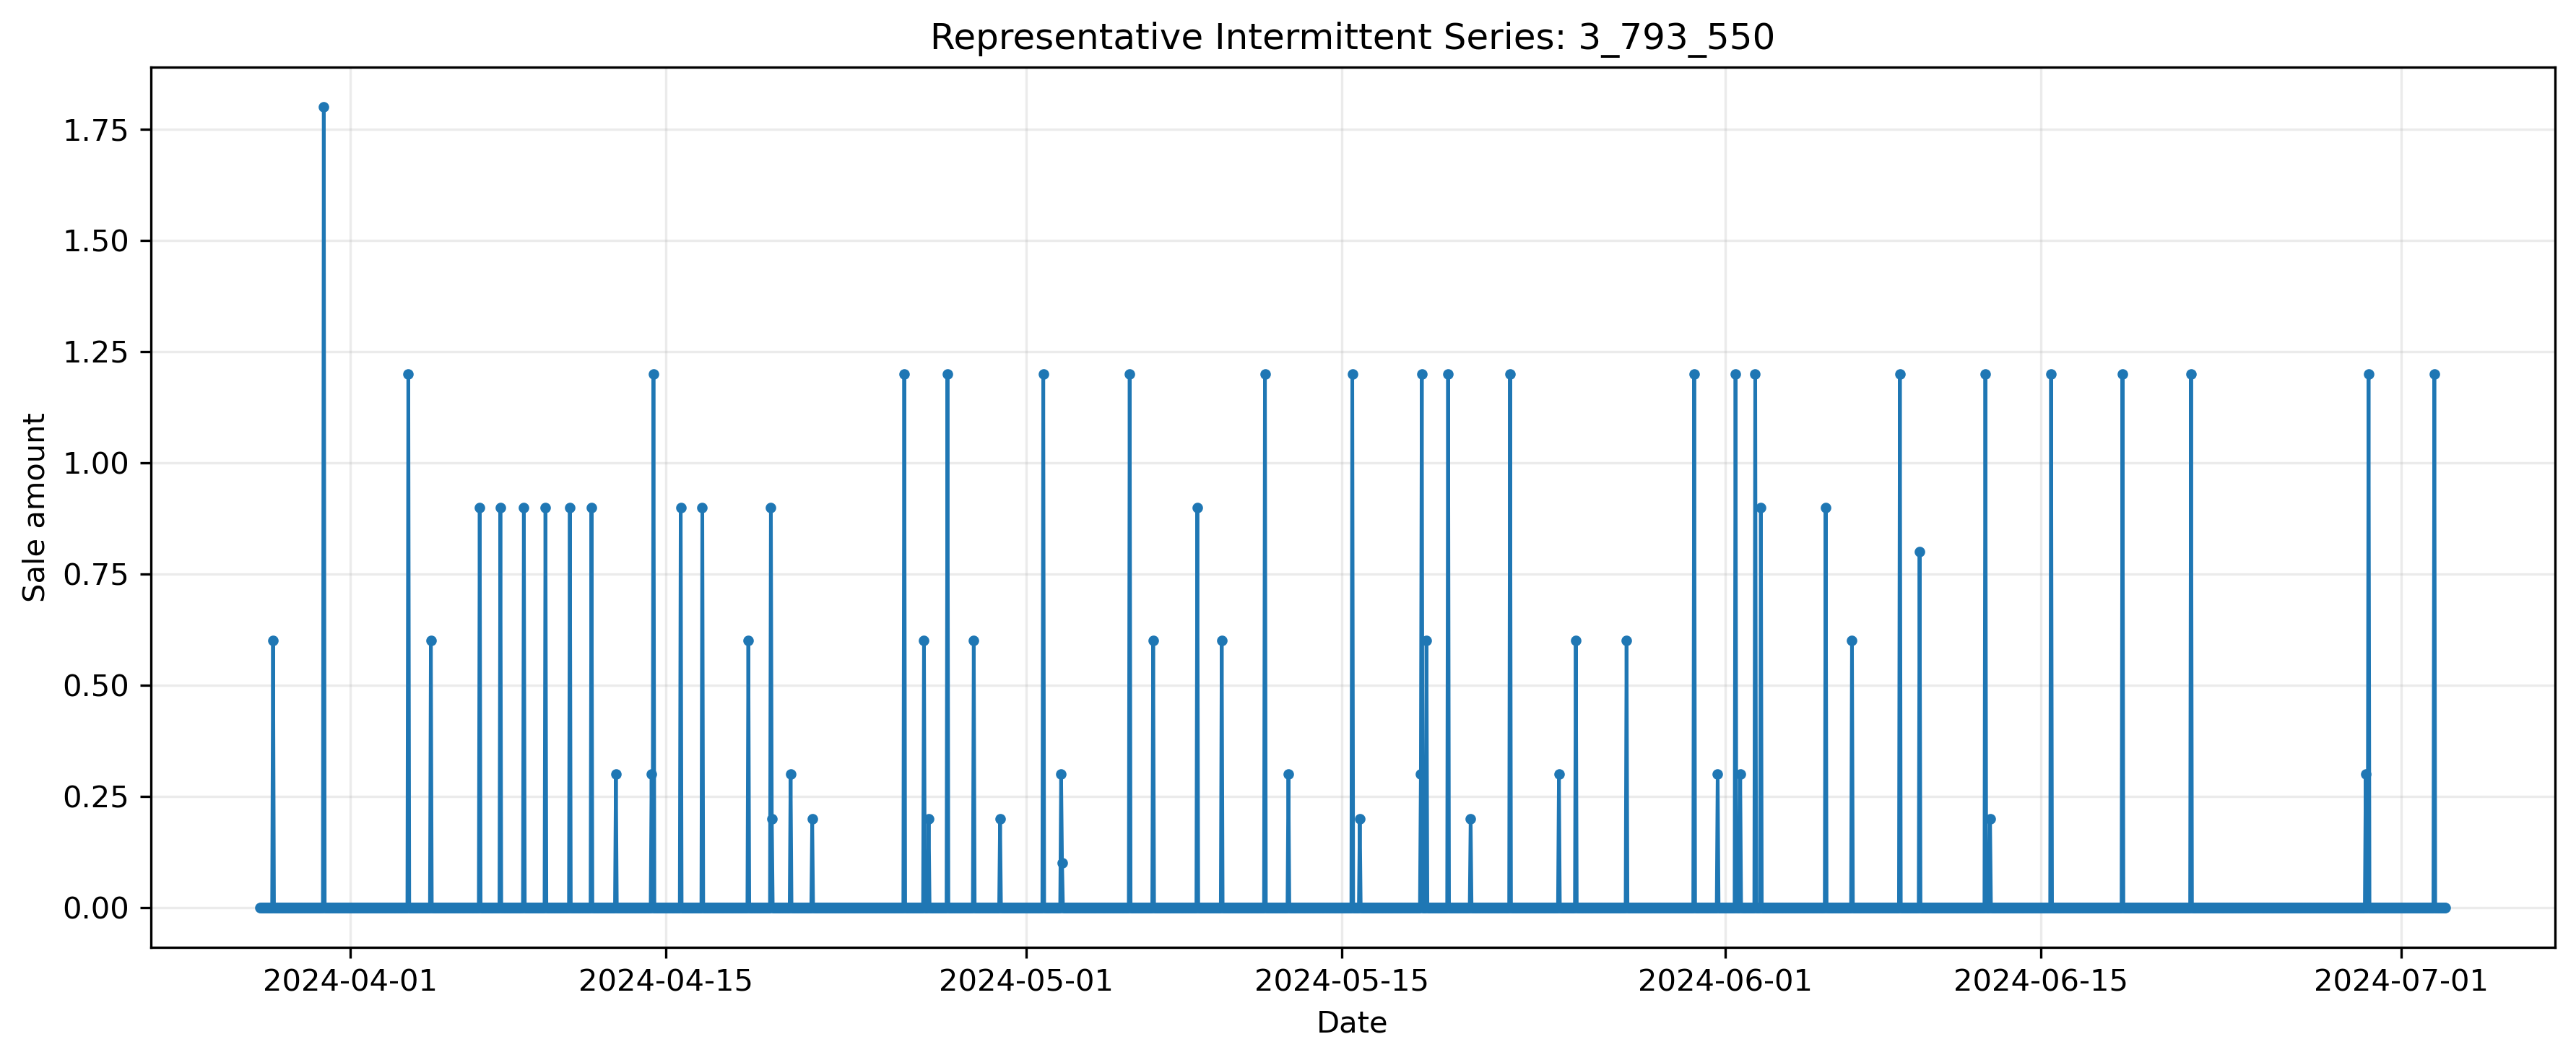
\includegraphics[width=0.92\linewidth]{figures/representative_series_intermittent.png}
    \caption{Chuỗi đại diện intermittent.}
    \label{fig:long-rep-intermittent}
\end{figure}



\begin{figure}[H]
    \centering
    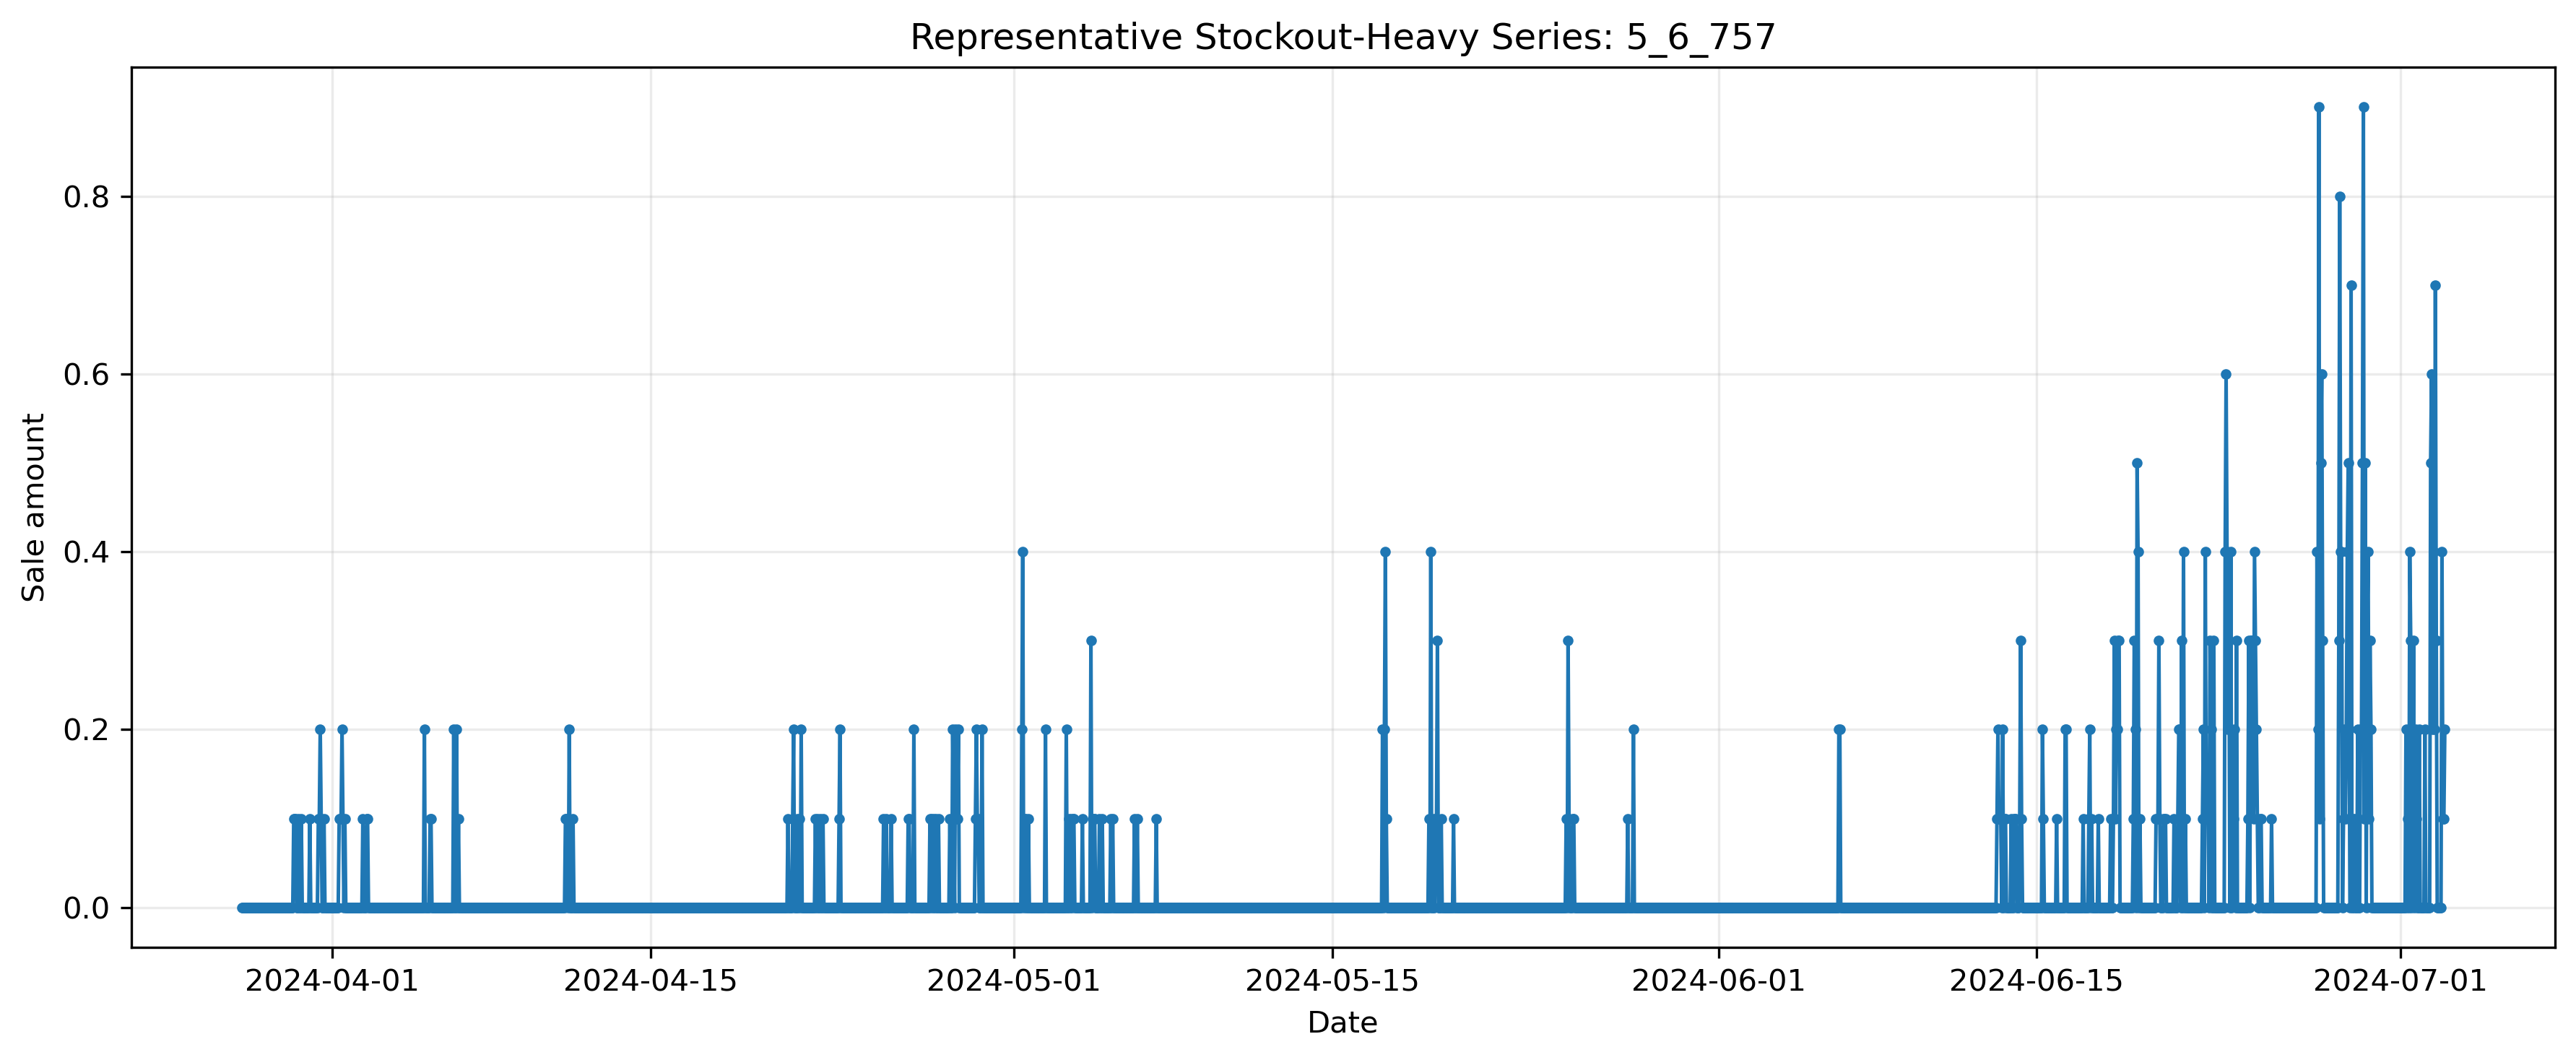
\includegraphics[width=0.92\linewidth]{figures/representative_series_stockout_heavy.png}
    \caption{Chuỗi đại diện stockout-heavy.}
    \label{fig:long-rep-stockout}
\end{figure}
